\subsection{Schwerpunktverteilung mit Integer}
\begin{table}[h!]
    \centering
    \begin{tabular}{ | c | c | c | c | c |}
        \hline
        & RandomForest & Boosting & Bagging & ExtraTrees \\\hline
        Maximalhöhe & 13 & 12 & - & 21 \\\hline
        Waldgröße & 15 & 14 & - & 11 \\\hline
        ccp\_alpha & 0.0 & 0.0 & - & 0.0 \\\hline
        min\_samples\_leaf & 4 & 4 & - & 2 \\\hline
        \textbf{Ohne Optimierung} &  &  &  &  \\\hline
        Größe in Bytes & - & - & - & - \\\hline
        Genauigkeit Klisch & 96.9\% & 92.7\% & - & 95.8\% \\\hline
        Genauigkeit Dymel Gesture & 98.0\% & 97.8\% & - & 98.8\% \\\hline
        Genauigkeit Dymel Null & 93.9\% & 93.6\% & - & 95.6\% \\\hline
        \textbf{Mit Optimierung} &  &  &  &  \\\hline
        Größe in Bytes & - & - & - & - \\\hline
        Genauigkeit Klisch & - & - & - & - \\\hline
        Genauigkeit Dymel Gesten & - & - & - & - \\\hline
        Genauigkeit Dymel Null & - & - & - & - \\\hline
    \end{tabular}
    \caption{Beste Konfigurationen je Ensemble-Methode der Schwerpunktverteilung mit Integer.}
    \label{tab:schwerpunktverteilung_int}
\end{table}
\begin{figure}[h!]
    \centering
    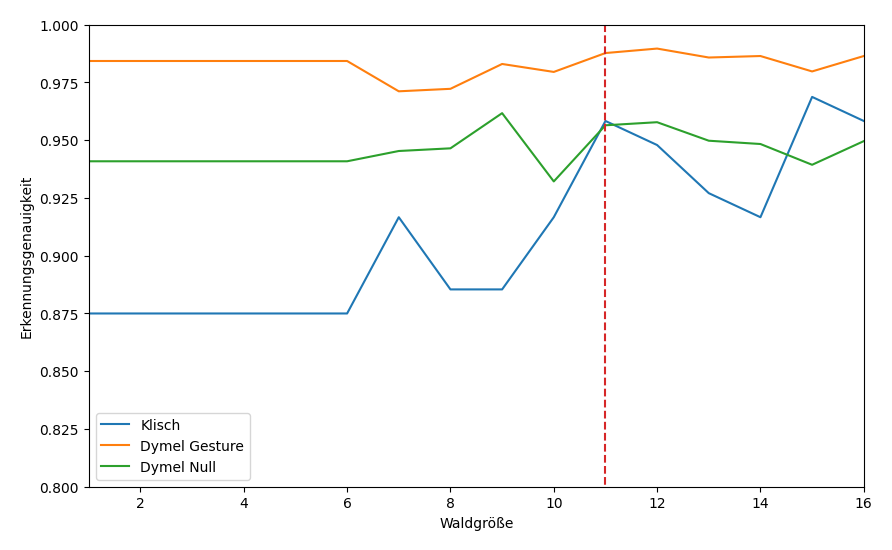
\includegraphics[width=\linewidth]{images/cocd_int_acc_per_size.png}
    \caption{Die beste summierte Erkennungsgenauigkeit pro Waldgröße der Schwerpunktverteilung mit Integer.}
    \label{fig:cocd_int_per_forest_size}
\end{figure}
Die Featuremenge Schwerpunktverteilung mit Integer folgt der Definition aus Sektion \ref{sec:schwerpunktverteilung} und beinhaltet insgesamt 10 Einträge, wobei jeweils 2 Einträge die X und Y
Koordinate des Schwerpunktes darstellen in insgesamt 5 Zeitfenstern. Anders als die Schwerpunktverteilung mit Gleitkommazahlen wird diese nicht durch die Summe aller Pixel dividiert, wodurch
X und Y zwischen -3072 und 3072 liegen anstatt -1 und 1.
\newline
\newline
Auch bei diesem Ansatz, weisen alle Ensemble-Methoden nur marginale Unterschiede auf (siehe Tabelle \ref{tab:schwerpunktverteilung_int}) im Hinblick auf die Erkennungsgenauigkeit. Insgesamt ist
die Konfigurationen mit ExtraTrees am besten, da die summierte Erkennungsgenauigkeit dort maximal ist. Der RandomForest hat aber die höchste Erkennungsgenauigkeit auf der Testmenge von Klisch.
Mit $96,9\%$ ist das noch besser als die Schwerpunktverteilung mit Gleitkommazahlen und $0,1\%$ besser als die beste Lösung die mit einer kleineren Trainingmenge ohne Nullgesten gefunden wurde.
\newline
\newline
Leider ist die Programmgröße aller Konfigurationen, ohne Optimierungen, zu groß um kompeliert zu werden. Zurzeit nutzt der Ansatz 32-Bit Integer. Als Optimierung wurde der Datentyp auf 16-Bit
Integer bzw. 8-Bit Integer reduziert und der hybride Wahlklassifizierer wurde genutzt. TODO: Reevaluierung.
\newline
\newline
Abbildung \ref{fig:cocd_int_per_forest_size} zeigt, dass die Erkennungsgenauigkeit der Testmengen mit zunehmender Waldgröße ebenfalls zunimmt. Wobei besonders die Erkennungsgenauigkeit der
Testmenge von Klisch stark schwankt.
